\documentclass[12pt]{article}
\usepackage[a4paper, total={5.5in, 9in}]{geometry}
\usepackage{amsmath}
\usepackage{amsfonts}
\usepackage{graphicx}
\usepackage{pgfplots}
\pgfplotsset{compat=1.18}
\usepackage{enumitem}

\title{College Algebra Worksheet 5.1}
\author{PCL Learning Center}
\date{}

\begin{document}
\maketitle

\begin{center}
    \textit{note: No graphing calculators or electronic devices may be used on this worksheet.}    
\end{center}

\section*{Problem Set 1\\Difficulty level: Normal}
\subsection*{Problem 1}
Determine the domain and range of the following parabola.
\[f(x)=-(x+5)^2-4\]

\subsection*{Problem 2}
An object is launched directly in the air at a speed of 144 feet per second from a platform located 12 feet in the air. The motion of the object can be modeled using the function \( f(t) = -16t^2 + 144t + 12 \), where \( t \) is the time in seconds and \( f(t) \) is the height of the object. When, in seconds, will the object reach its maximum height?

\subsection*{Problem 3}
Find the \(x\)-intercept(s) of the following function.
\[f(x)=10x^2+23x-42\]

\subsection*{Problem 4}
An archer releases an arrow with an initial velocity of 24 feet per second at a height of 16 feet. The path the arrow takes can be modeled using the function \( f(t) = -16t^2 + 24t + 16 \), where \( f(t) \) represents the height, in feet, of the arrow and \( t \) represents the time the arrow travels in seconds. How many seconds until the arrow hits the ground? Round your answer to the nearest hundredth if necessary. Do not include units in your answer.

\subsection*{Problem 5}
In interval notation, express the set of all numbers greater than \(-10\) and less than \(-3\).

\subsection*{Problem 6}
Determine the direction in which the graph of the following parabola opens.
\[f(x)=x^2-10x+24\]
\begin{enumerate}
    \item[(a)] Up
    \item[(b)] Down
    \item[(c)] Left
    \item[(d)] Right
\end{enumerate}

\subsection*{Problem 7}
Determine the vertex of the graph of the following parabola.
\[f(x)=-(x-3)^2-3\]

\subsection*{Problem 8}
Determine the axis of symmetry of the parabola whose graph is given below. Your answer should be in the form \(x=h\).

\begin{center}
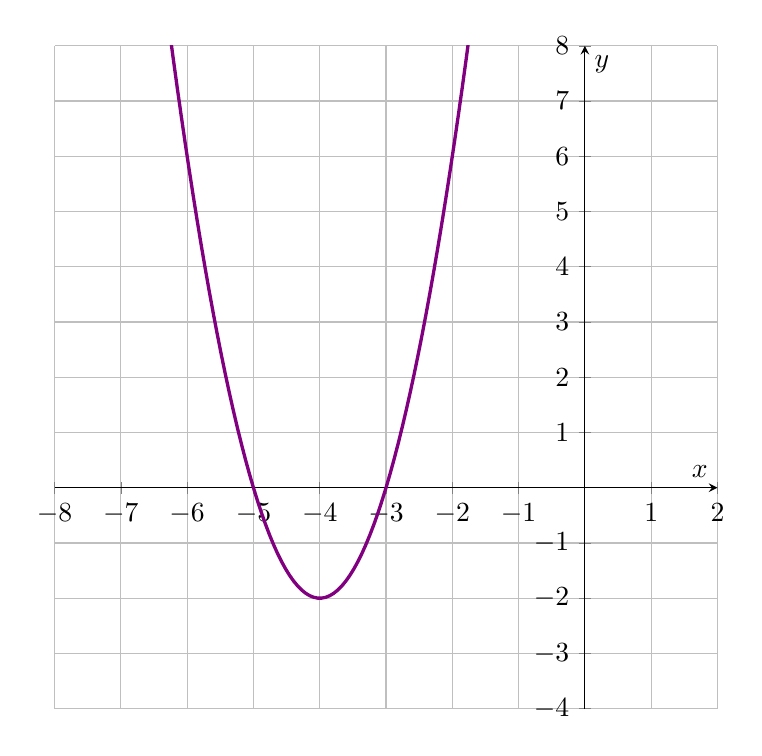
\begin{tikzpicture}
\begin{axis}[
    axis lines=middle,
    width=10cm,
    height=10cm,
    xmin=-8, xmax=2,
    ymin=-4, ymax=8,
    xtick={-8,...,2},
    ytick={-4,...,8},
    grid=both,
    xlabel=\(x\),
    ylabel=\(y\),
]
\addplot[domain=-7:-1, samples=100, very thick, violet] {2*(x + 4)^2 - 2};
\end{axis}
\end{tikzpicture}
\end{center}

\subsection*{Problem 9}
Determine the \(x\)-intercepts of the parabola whose graph is given below.

\begin{center}
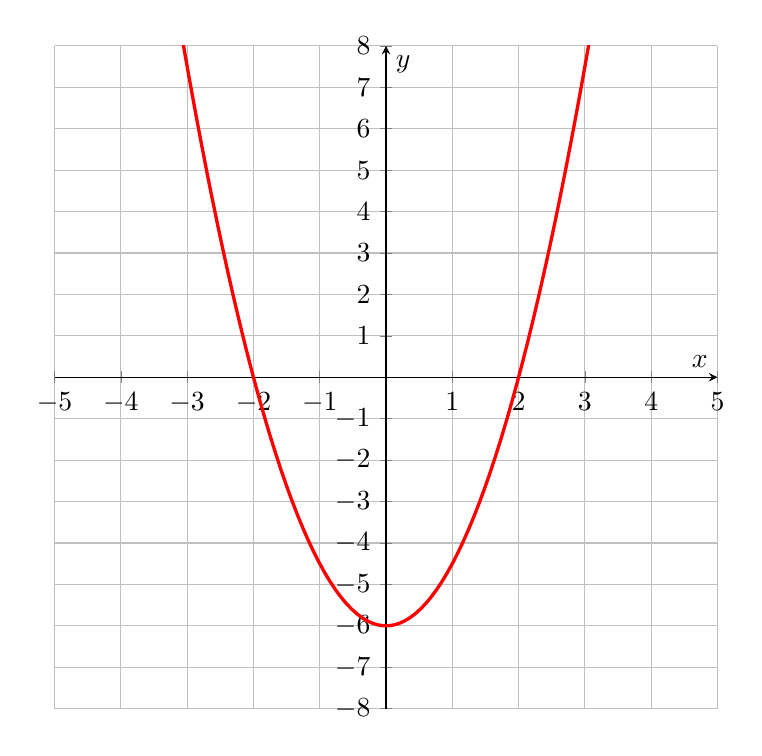
\begin{tikzpicture}
\begin{axis}[
    axis lines=middle,
    width=10cm,
    height=10cm,
    xmin=-5, xmax=5,
    ymin=-8, ymax=8,
    xtick={-5,...,5},
    ytick={-8,...,8},
    grid=both,
    xlabel=\(x\),
    ylabel=\(y\),
]
\addplot[domain=-4:4, samples=100, very thick, red] {1.5*x^2 - 6};
\end{axis}
\end{tikzpicture}
\end{center}

\subsection*{Problem 10}
Determine the equation of the parabola whose graph is given below.\\
\textit{note: Some points of the parabola are \((-1,0),(4,0),(0,-4), \text{ and } (3,-4)\)}

\begin{center}
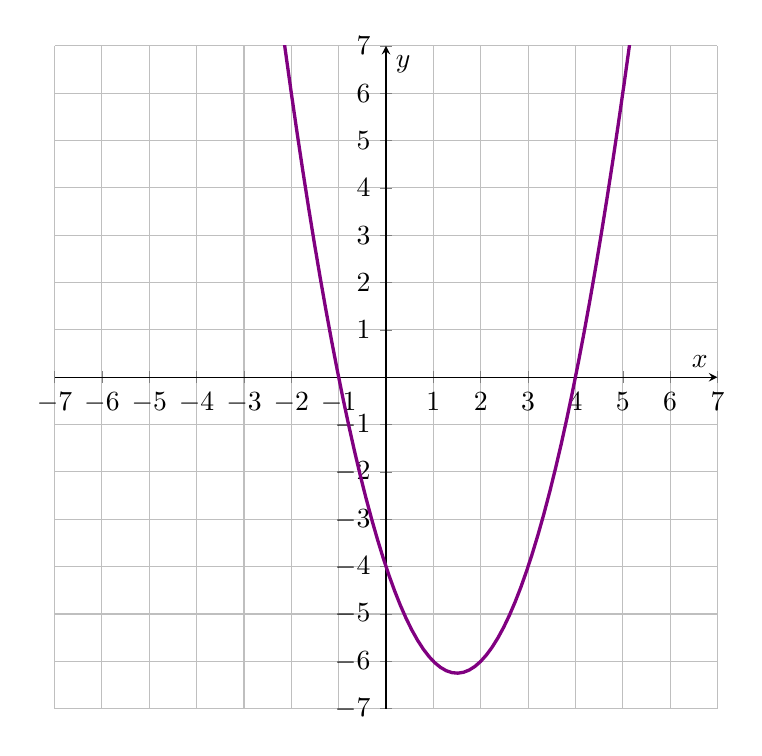
\begin{tikzpicture}
\begin{axis}[
    axis lines=middle,
    width=10cm,
    height=10cm,
    xmin=-7, xmax=7,
    ymin=-7, ymax=7,
    xtick={-7,...,7},
    ytick={-7,...,7},
    grid=both,
    xlabel=\(x\),
    ylabel=\(y\),
]
\addplot[domain=-6:6, samples=100, very thick, violet] {x^2 - 3*x - 4};
\end{axis}
\end{tikzpicture}
\end{center}

\subsection*{Problem 11}
Write and equation for the parabola whose graph is given below.\\
\textit{note: Some points of the parabola are \((-5,5),(-3,5), \text{ and } (-4,3)\)}

\begin{center}
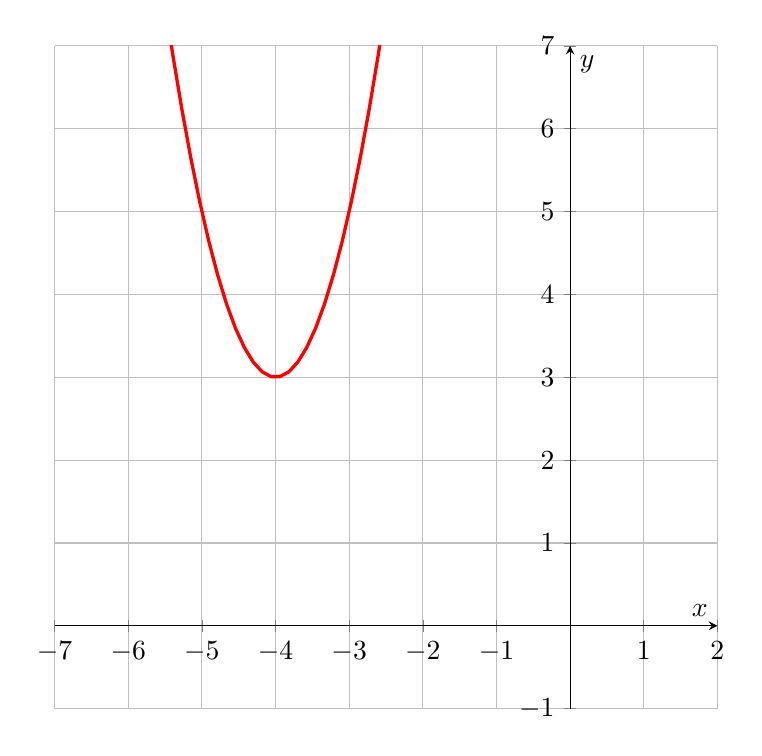
\begin{tikzpicture}
\begin{axis}[
    axis lines=middle,
    width=10cm,
    height=10cm,
    xmin=-7, xmax=2,
    ymin=-1, ymax=7,
    xtick={-7,...,2},
    ytick={-1,...,7},
    grid=both,
    xlabel=\(x\),
    ylabel=\(y\),
]
\addplot[domain=-6:6, samples=100, very thick, red] {2*(x+4)^2+3};
\end{axis}
\end{tikzpicture}
\end{center}

\subsection*{Problem 12}
Rewrite the following quadratic function in vertex form \(f(x)=a(x-h)^2+k\).
\[f(x)=6x^2+2x-5\]

\subsection*{Problem 13}
A farmer is building a fence to enclose a rectangular area against an existing wall, shown in the figure below.\\
\begin{figure}[!ht]
    \centering
    \includegraphics[width=0.5\linewidth]{6.png}
\end{figure}

Three of the sides will require fencing and the fourth wall already exists. If the farmer has 144 feet of fencing, what are the dimensions of the region with the largest area?

\newpage
\section*{Solutions to the Set 1}
\subsection*{Problem 1}
Domain is all real numbers. Range is \(f(x) \leq -4\).
\subsection*{Problem 2}
\(4.5\)
\subsection*{Problem 3}
\((-\dfrac{7}{2},0)\) and \((\dfrac{6}{5},0)\)
\subsection*{Problem 4}
2
\subsection*{Problem 5}
\((-10,-3)\)
\subsection*{Problem 6}
\begin{enumerate}
    \item[(a)] Up 
\end{enumerate}
\subsection*{Problem 7}
\((3,-3)\)
\subsection*{Problem 8}
\(x=-4\)
\subsection*{Problem 9}
\((-2,0),(2,0)\)
\subsection*{Problem 10}
\(f(x)=x^2-3x-4\)
\subsection*{Problem 11}
\(f(x)=2x^2+16x+35\)
\subsection*{Problem 12}
\(f(x)=6(x+\dfrac{1}{6})^2-\dfrac{31}{6}\)
\subsection*{Problem 13}
36 feet by 72 feet.

\end{document}
